\documentclass[tog]{acmsiggraph}
\graphicspath{{./images/}}
\usepackage{gensymb}
\usepackage[ngerman]{babel}
\usepackage[utf8]{inputenc}
\usepackage[T1]{fontenc}
\usepackage{hyperref}
\usepackage{listings}
\usepackage{amsmath}
\newcommand{\code}[1]{\texttt{#1}}
%%% Make the ``BibTeX'' word pretty...
\def\BibTeX{{\rm B\kern-.05em{\sc i\kern-.025em b}\kern-.08em
    T\kern-.1667em\lower.7ex\hbox{E}\kern-.125emX}}

%%% Used by the ``review'' variation; the online ID will be printed on 
%%% every page of the content.

\TOGonlineid{00001}

%%% Used by the ``preprint'' variation.

\TOGvolume{0}
\TOGnumber{0}

\title{Übung 1 - Computergrafik-I, WS 2015/16}
\author{Christoph Stumpe, Fabian Wendland, Martin Zier\\Beuth Hochschule für Technik Berlin}
\pdfauthor{Martin Zier, s59330}
\date{25. Oktober 2015}

\keywords{Matrizen, Mathematik, Java Übung}

\begin{document}
\iffalse
 \teaser{
   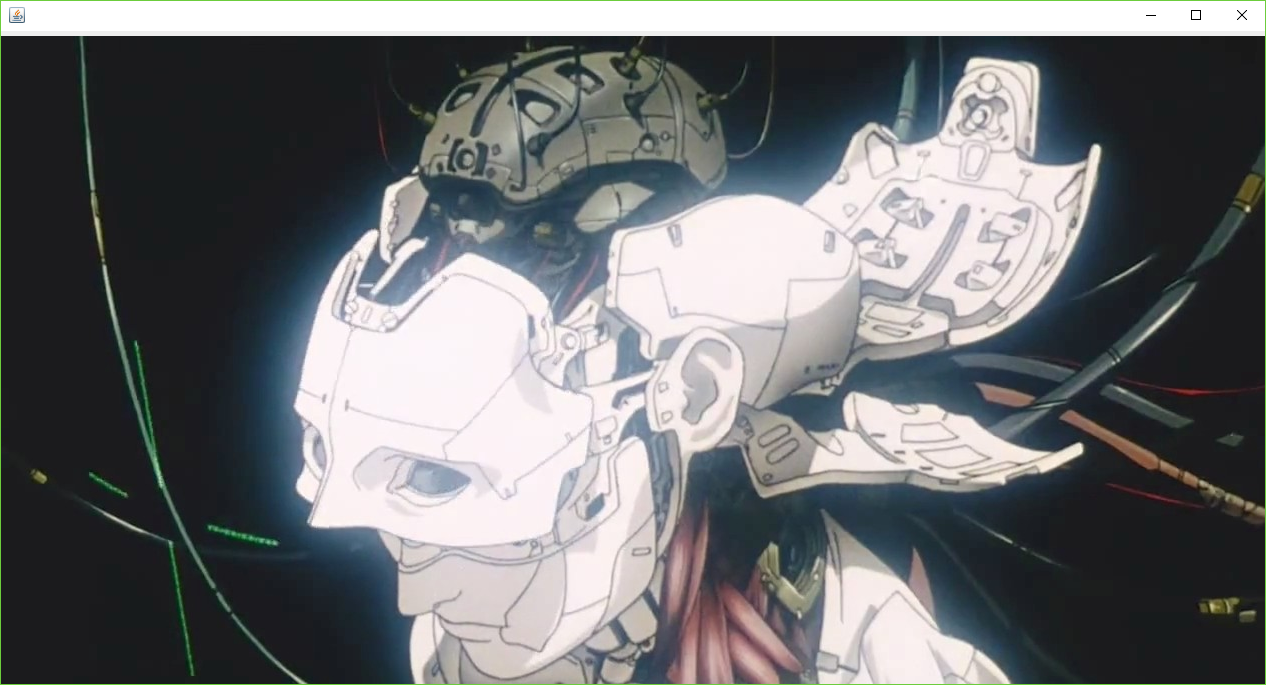
\includegraphics[height=2in]{01_image-frame.png}
   \caption{Vorbereitungsübung 1 -- Quelle: \textsc{Ghost in the Shell}, 1996}
 }
\maketitle
\fi
\tableofcontents
\newpage

\section{Einführung}
Dies ist die Mitschrift vom 03.11.2015 von Computergrafik I. In der Vorlesung behandelten wir erste geometrische Formeln, welche relevant für den weiteren Verlauf der Entwicklung eines Raytracers sind. Neben den Grundlagen, die unter anderem Schnittberechnung und implizierte Oberflächen behandelten, ging es des weiteren um die Ebene und die Kugel als geometrische Form. 

\section{Geometrien - Grundlagen}
Geometrische Formen kennen wir alle aus der Grundschule. Dreiecke, Kreise, Vierecke oder Rauten. Oft werden zweidimensionale Koordinatensysteme dafür genutzt, dreidimensionale Objekte in einem zweidimensionalen Raum darzustellen. Das ist auch für die virtuelle Darstellung von 3D Objekten relevant, denn zum Beispiel ist eine Kugel, die wir von einer Seite betrachten, auch nur ein Kreis. Die euklidische Geometrie, ist relevant für die weitere Arbeit an unseren Raytracern.

\section{Schnittpunkte - wenn Welten Kollidieren}

\begin{figure}[ht]
  \centering
	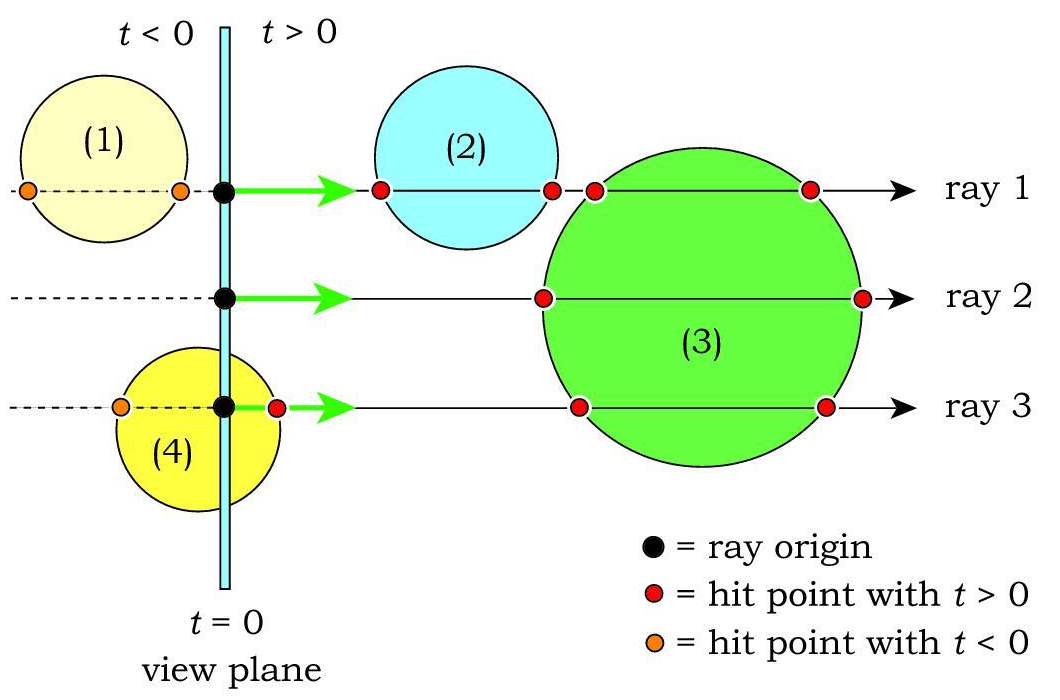
\includegraphics[width=3.2in]{mitschrift_schnittpunkte.png}
	\caption{Grundlegende Szene mit vier Kugeln}
  \label{fig:base_scene}
\end{figure}
Wir haben eine Kamera und vier Kugeln in verschiedenen Größen, Farben und Positionen. Die Kamera dient als unser POV (Point-of-View). Wenn nun Lichtstrahlen die Kamera verlassen, werden diese offensichtlich Objekte schneiden, die sich vor der Kamera befinden. Wir schießen für jeden Pixel in unserem Bild einen Strahl los. Zusätzlich haben wir noch die Variable $t$, die hier für unsere Sichtposition steht. $t = 0$ sind also wir, die Kamera. Sollte sich $t$ nun im negativen Bereich befinden, werden wir die Objekte nicht sehen, da diese sich hinter der Kamera befinden. Dementsprechend sehen wir Kugel 1 aus der Zeichnung nicht. Kugel 4 befindet sich zur Hälfte in unserem Sichtfeld und wird somit dargestellt, die Kugeln 2 und 3 ebenfalls. Da wir natürlich nicht durch Objekte durchschauen können (außer sie wären transparent), wollen wir lediglich die Kugeln an den Stellen rendern, dir wir auch wirklich sehen können. Deswegen suchen wir immer nach dem kleinsten $t$ für jedes Objekt, weil dieses offensichtlich die Vorderseite für uns darstellt. Anzumerken ist auch, dass Kugel 3 von 2 und 4 teilweise verdeckt werden, da diese sich vor der großen roten Kugel im Raum befinden.

\section{Ebenen}
\subsection{Implizite Oberflächen}
Um zu verstehen, was implizite Oberflächen bzw. Funktionen im Allgemeinen sind, sollten wir uns zuerst explizite Funktionen anschauen. Klassisch hätten wir da zum Beispiel $$f(x) = ax +b$$ Für jeden $x$-Wert, den wir in die Funktion stecken, bekommen wir einen expliziten $y$-Wert.\newline
Bei einer impliziten Funktion geben wir wiederum Werte an, um herauszufinden, ob der jeweilige Punkt auf der korrespondierenden Geraden liegt oder eben nicht. 
$$f(x,y,z) = 0$$
Für unsere impliziten Oberflächen bedeutet dies nun im Folgeschluss, dass $f(\vec{p}) = 0$ uns sagt, ob der jeweilige Punkt auf der Oberfläche liegt oder nicht. $f(\vec{p}) = 0$ bedeutet, dass der Punkt auf der Oberfläche liegt. Da unser Strahl uns für jedes $t$ einen Punkt gibt, können wir daraus schließen:
$$f(\vec{o} + t\vec{d}) = 0$$ $t$ ist nun die einzige unbekannte Variable, welche wir durch umstellen errechnen können. 

\subsection{Implizite Ebenen}

\begin{figure}[ht]
  \centering
	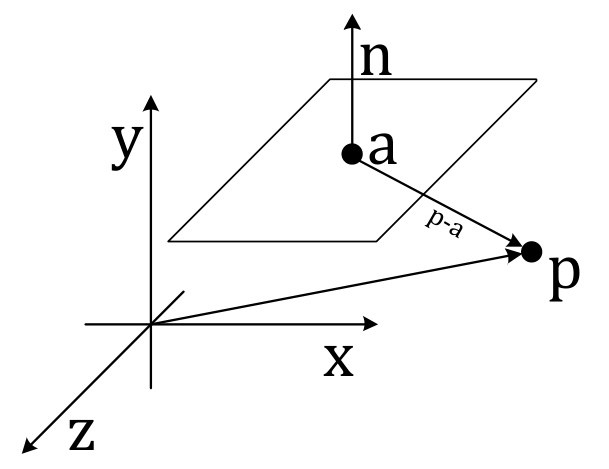
\includegraphics[width=3.2in]{mitschrift_implizite_ebene.png}
	\caption{Darstellung einer impliziten Ebene in Koordinatensystem}
  \label{fig:implicit_plane}
\end{figure}
Um eine implizite Ebene in einem Raum darstellen zu können, brauchen wir zwei Werte. Wir brauchen Vektor $a$, einen uns bekannten Punkt und Vektor $n$, die Normale, welche uns sagt, wie die Ebene ausgerichtet ist. Um nun herauszufinden, ob ein Punkt auf der Ebene liegt, müssen wir lediglich feststellen, ob die Normale in einem $90\degree$ Winkel auf dem Punkt steht. Um das herauszufinden, wenden wir folgende Gleichung an: 
$$(\vec{p} - \vec{a}) \cdot \vec{n} = 0$$ 
Da wir mit Strahlen, mit unseren Rays, arbeiten, wird aus der Formel:
$$(\vec{o}+t\cdot\vec{d}-\vec{a})\cdot\vec{n} = 0$$
Das müssen wir nun nach $t$ auflösen, da $t$ unsere Unbekannte ist:
$$\vec{o}\cdot\vec{n} + t\vec{d}\cdot\vec{n} - \vec{a} \cdot \vec{n} = 0$$
Jetzt stellen wir die Formel noch um:
$$t\vec{d}\cdot\vec{n} = \vec{a}\vec{n} - \vec{o}\vec{n}$$
Jetzt lösen wir $d$ und $n$ noch vom $t$ und wir sind fast fertig:
$$t = \frac{\vec{a}\cdot\vec{n} - \vec{o} \cdot \vec{n}}{\vec{d}*\vec{n}}$$
Wir können nun noch das n ausklammern und erhalten somit unsere finale Formel für die implizite Ebene:
$$t = \frac{(\vec{a}-\vec{o}) \cdot \vec{n}}{\vec{d}\cdot\vec{n}}$$

\section{Kugel}

\end{document}